%%%%%%%%%%%%%%%%%%%%%%%%%%%%%%%%%%%%%%%%%
% Homework Assignment - REEU2021
% LaTeX Template
% Version 1.0 (02/10/2021)
%
%
% Author:
% Justin A. Gould (gould29@purdue.edu)
%
% License:
% CC BY-NC-SA 3.0 (http://creativecommons.org/licenses/by-nc-sa/3.0/)
%
%%%%%%%%%%%%%%%%%%%%%%%%%%%%%%%%%%%%%%%%%

%----------------------------------------------------------------------------------------
%	PACKAGES AND OTHER DOCUMENT CONFIGURATIONS
%----------------------------------------------------------------------------------------

\documentclass{homework}
\usepackage{verbatim}
\usepackage{graphicx}

%----------------------------------------------------------------------------------------
%	COURSE AND INSTRUCTOR INFORMATION
%----------------------------------------------------------------------------------------

\HWauthor{Justin A. Gould}{gould29@purdue.edu}
\HWno{1}
\HWcourse{REEU 2021}

\begin{document}
\maketitle

%----------------------------------------------------------------------------------------
%	INSTRUCTIONS
%----------------------------------------------------------------------------------------

\textbf{Instructions}

All files and data you need to complete this assignment are:
\begin{itemize}
    \item \verb|UScounties|: A folder containing a shapefile (and supporting files) for the \verb|POLYGON| of every U.S. county.
    \item \verb|covid_us_counties.csv|: A CSV of county-level COVID-19-related data from January 2020 through February 2021.
    \item \verb|co-est2019-alldata.csv|: A CSV of the population of every U.S. county, organized by FIPS code.
\end{itemize}

\clearpage

%----------------------------------------------------------------------------------------
%	TASK AND DATA SUMMARY
%----------------------------------------------------------------------------------------

\textbf{Data Overview and Task Requirements}\\
Your task is to create a choropleth map of COVID-19 case data for the domestic United States. Specifically, you're tasked with calculating and mapping the 7-day moving average of new cases per 100,000 residents on November 03, 2020.\\



\textbf{HINT}: I suggest working in Python first, as we did in class, to do the preprocessing, before moving to QGIS for the second question.\\

\begin{figure}
    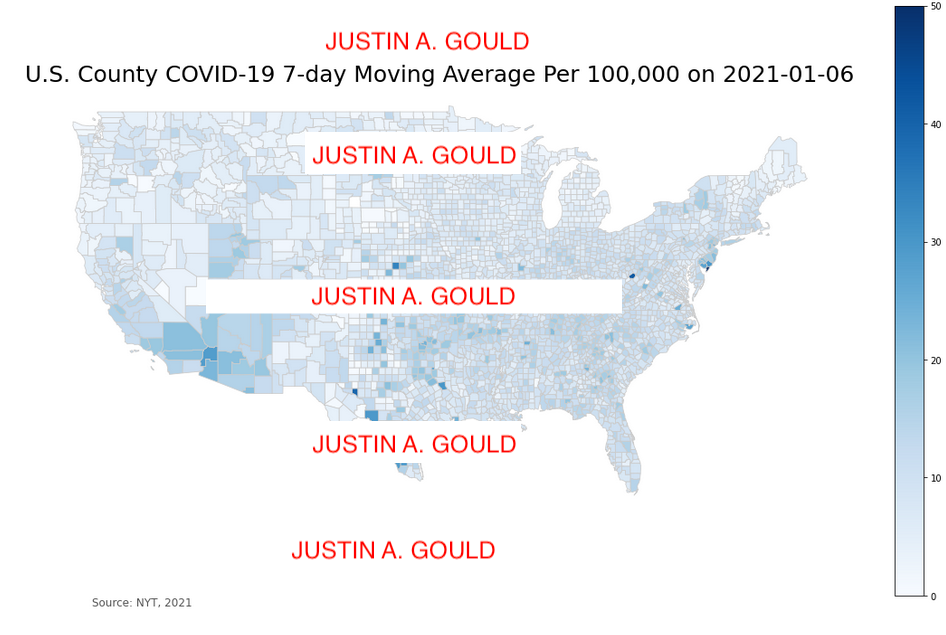
\includegraphics[width=\linewidth]{./final_map.png}
    \caption{Example map output}
    \label{fig:final_map}
\end{figure}

Your final map should look something like Figure \ref{fig:final_map}. \\

\textbf{Preprocessing Steps}:
\begin{itemize}
    \item Remove counties from Hawaii and Alaska from the shapefile.
    \item Calculate daily case increases at the FIPS code level.
    \item Calculate 7-day moving average of daily increase in cases at the FIPS code level...\textbf{HINT}: There is a built-in function in the \verb|pandas| package you can use to do this!
    \item \verb|JOIN| the following data into one Pandas DataFrame: FIPS geometry, NYT COVID-19 case data (your calculations), FIPS population data.
    \item Finally, be sure to filter the final DataFrame to show only the target date.
\end{itemize}

\clearpage

%----------------------------------------------------------------------------------------
%	QUESTION 1
%----------------------------------------------------------------------------------------

\HWproblem
\textbf{Visualizing a COVID Map via Python}\\
Create a choropleth map of 7-day average of new cases per 100,000 residents on November 03, 2020, via \verb|pandas|, \verb|geopandas|, and \verb|matplotlib|.\\

\textbf{Input:} The data and files described on page 2.\\

\textbf{Desired Output:} Please submit your \verb|.ipynb| and image of the map (either as \verb|.png| or \verb|.pdf|). Your notebook \textbf{must} show the \verb|GeoDataFrame| used to generate the map.\\


%----------------------------------------------------------------------------------------
%	QUESTION 2
%----------------------------------------------------------------------------------------

\HWproblem
\textbf{Visualizing a COVID Map via QGIS}\\
Create a choropleth map of 7-day average of new cases per 100,000 residents on November 03, 2020, via \verb|QGIS|.\\

\textbf{Input:} The data and files described on page 2.\\

\textbf{Desired Output:} Please submit your QGIS project as a \verb|.qgz| file and image of the map (either as \verb|.png| or \verb|.pdf|).

\clearpage

\end{document}